\documentclass[a4paper,11pt]{book}
\setlength{\topmargin} {1 cm}
\setlength{\footskip} {0 cm}
\usepackage [T1]{fontenc}
\usepackage [utf8]{inputenc}
\usepackage [italian]{babel}
\usepackage {graphicx}
\usepackage {frontespizio}
\usepackage[a4paper, total={6in, 9in}]{geometry}

\begin{document}

\begin{frontespizio}
\Logo{logo.jpg}
\Universita{Verona}
\Facolta{Scienze e Ingegneria}
\Corso[Laurea]{Informatica}
\Titolo{Progetti Basi di dati - G30}
\Candidato[VR359333]{Falda Alessandro}
\Candidato[VR359129]{Marini Alberto}
\Annoaccademico{2013 - 2014}
\end{frontespizio}

\tableofcontents

\chapter{Progetto}

\section{Requisiti}
Si vuole progettare un sistoma informativo per gestire l'emissione di biglietti di una compagnia di autobus extraurbani.
Il sistema gestisce l'emissione di quattro tipi di biglietti: le corse semplici, la corsa andata e ritorno, gli abbonamenti settimanali e gli abbonamenti mensili. 
Ogni biglietto è univocamente identificato da un codice di emissione. Inoltre per ogni biglietto emesso si registra: la linea, la fermata di partenza di partenza e quella di arrivo, l'importo e la data di emissione. 
Per gli abbonamenti si registra  in aggiunta la data di inizio validità, la data di fine validità e i dati del cliente intestatario: codice fiscale, nome, cognome, data di nascita e comune di residenza. 
Ogni cliente può essere titolare di più abbonamenti. 
L'emissione dei biglietti avviene a fronte di un credito che il cliente ottiene versando un certo importo presso gli sportelli della società.
Per ogni versamento il sistema registra: il cliente che l'ha eseguito, l'importo del versamento e la data e l'ora in cui è avvenuto.
Un cliente può acquistare biglietti e/o abbonamenti solo se ha un saldo attivo tra versamenti eseguiti e biglietti comprati. Per ogni biglietto acquistato il sistema registra in aggiunta il cliente che l'ha acquistato (per gli abbonamenti, l'acquirente potrebbe essere diverso dall'intestatario dell'abbonamento).
Per eseguire gli acquisti a ogni cliente viene assegnatea una coppia: login e password.
Ogni linea coperta dagli autobus è caratterizzata da un codice univoco, il capolinea di partenza, il capolinea di arrivo e la durata media della percorrenza.
Ogni corsa è caratterizzata da: una linea, un senso di marcia (diretto/inverso), un orario di partenza e un orario di arrivo.
Si memorizzano infine gli orari delle corse che coprono le varie linee indicando tutte le fermate e per ogni fermata l'orario di arrivo alla fermata.
Si suppone che gli orari siano fissati e invariati per tutto l'anno solare.

\chapter{Sito web}
\section{Reguititi}
Le informazioni contenute nella basi di dati devono essere presentate in un sito web. Tale sito deve essere strutturato in schemi di pagina come di seguito descritto; è possibile estendere la struttura aggiungendo ulteriori schemi di pagina che mostrano ulteriori dettagli:
\begin{itemize}
\item HomePage, dove si riporta:
	\begin{itemize}
	\item La presentazione della società di trasporto
	\item Foto della società
	\item Contatti
	\item Una form che richiede login e password dell'utente per l'accesso alle pagine riservate per gli acquisti dei biglietti (UtentePage)
	\item Un link alla pagina degli orari (OrariPage)
	\end{itemize}
\item OrariPage, dove si mostra l'elenco di tutte le linee riportando per ogni linea: il codice, il capolinea di partenza e il capolinea di arrivo. Il codice è un link verso lo schema di pagina LineaPage.
\item LineaPage, dove si mostrano tutte le informazioni su una linea e l'elenco di tutte le corse della linea divise in due liste: le corse dirette e quelle in senso inverso. In ogni lista si riporta per ogni corsa: l'orario di partenza, l'orario di arrivo e per ogni corsa l'elenco delle fermate con gli orari di arrivo alla fermata.
\item UtentePage, dove si mostrano tutti i dati del cliente. L'elenco dei versamenti eseguiti dove si riporta: la data del versamento e l'importo versato. L'elenco dei biglietti acquistati divisi per tipologia, dove si riporta il codice del biglietto e la data di emissione. Il codice è un link verso lo schema di pagina BigliettoPage. Si aggiunge un link alla pagina AcquistoBigliettoPage. Tale link deve essere attivo solo se il saldo dell'utente è positivo.
\item BigliettoPage, dove si mostrano tutti i dati di un biglietto.
\item AcquistoBigliettoPage, dove si mostra una form per raccogliere i dati per l'acquisto di un biglietto. Alla pressione del bottone submit il sistema registra il biglietto nel sistema.
\end{itemize}

\chapter{Progetto concettuale}
\begin{figure}[!ht]
\centering
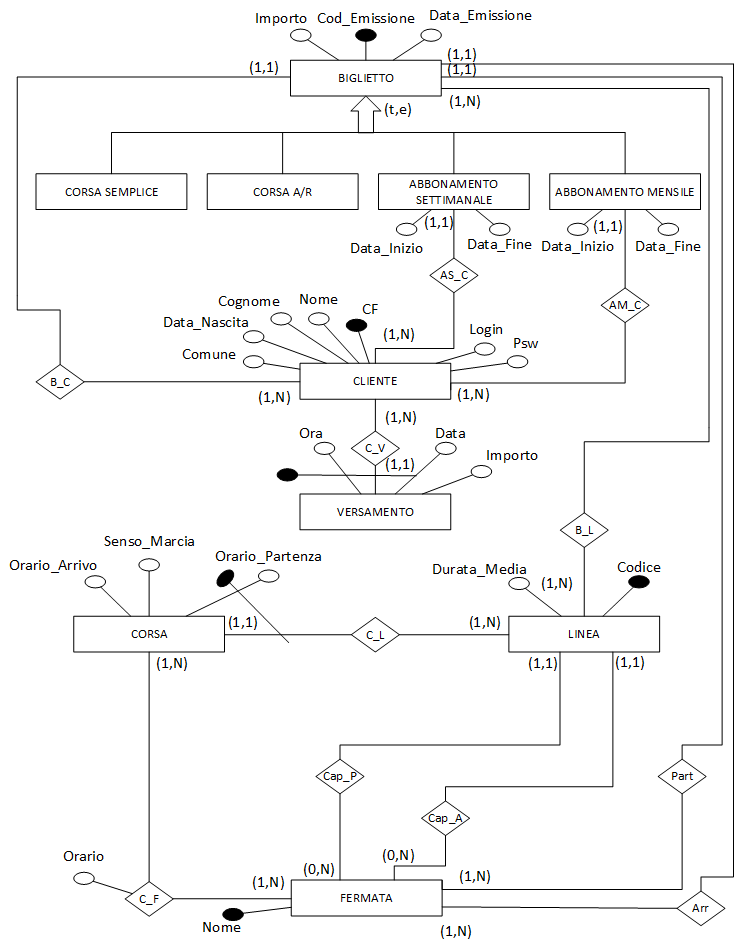
\includegraphics[scale = 0.3]{ER.png}
\caption{ER}
\end{figure}

\clearpage
Dopo aver risolto la generalizzazione, il nuovo schema Entità Relazioni risulta essere il seguente

\begin{figure}[!ht]
\centering
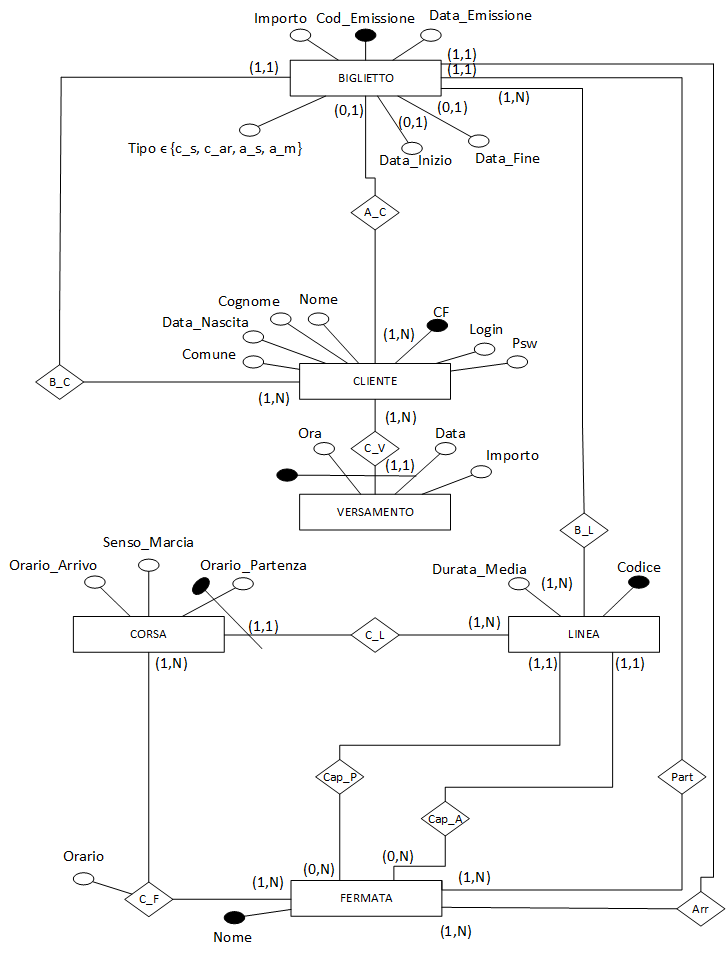
\includegraphics[scale = 0.3]{Generalizzazione.png}
\caption{Generalizzazione}
\end{figure}

\chapter{Schema Relazionale}

\begin{figure}[!ht]
\centering
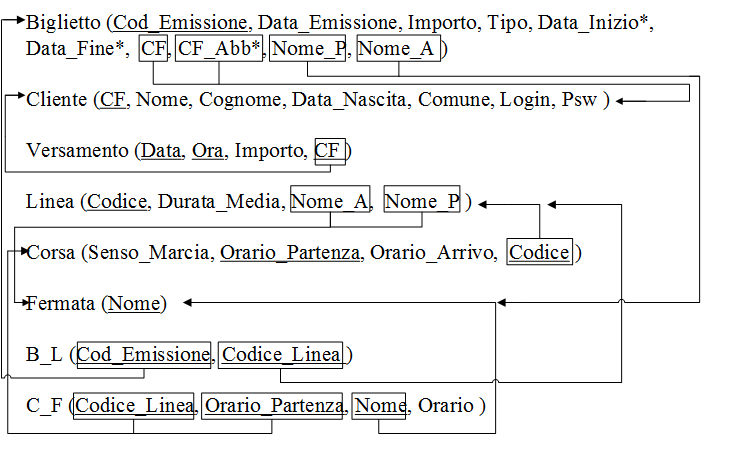
\includegraphics[scale = 0.3]{Schema_Relazionale.png}
\caption{Schema_Relazionale}
\end{figure}

\chapter{Struttura applicazione web}
La \figurename ~\ref{fig:struttura} mostra la struttura dell’applicazione web creata per il progetto. Abbiamo utilizzato l'architettura MVC-2 con un approccio Servlet-centric e l'aggiunta di Hibernate 
Abbiamo la parte di Model (parte logica) che interagisce con il DBMS creato estraendone le informazioni di interesse, tramite le classi DBMS.java e i JavaBeans. L'interazione con il database viene effettuata utilizzando Hibernate. Il modulo Controller (flusso) è sappresentato dalle servlet Main.java e AjaxServlet.java, che hanno il compito di prendere le informazioni che arrivano dal modulo precedente e trasferirle a chi si preoccupa della visualizzazione. La servlet 'AjaxServlet.java' viene utilizzata dalla form presente in AcquistoPage per il controllo scritto in Ajax. Infine l’ultima parte di View (presentazione) è gestita dalle JSP che indicano il modo di mostrare i dati all’utente finale dell’applicazione.


\begin{figure}[!ht]
\centering
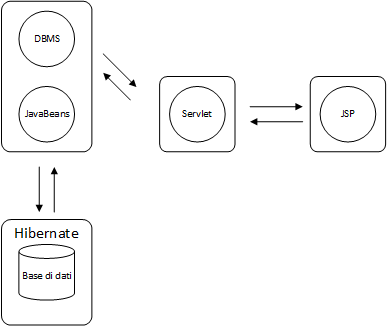
\includegraphics[scale = 0.3]{Struttura.png}
\caption{Struttura}
\label{fig:struttura}
\end{figure}

Nel nostro progetto: 
\begin{itemize}
\item la parte del DBMS è svolta da DBMS.java 
\item i JavaBeans sono: BigliettoBean.java, C_FBean.java, ClienteBean.java, CorsaBean.java, FermataBean.java, LineaBean.java e Versamentobean.java
\item per la parte di hibernate, sono stati creati: BigliettoBean.hbm.xml, C_FBean.hbm.xml, ClienteBean.hbm.xml, CorsaBean.hbm.xml, FermataBean.hbm.xml, LineaBean.hbm.xml e Versamentobean.hbm.xml
\item le servlet sono: Main.java e AjaxServlet.java
\item le JSP sono: Index.html, Utente.jsp, Orari.jsp, Linea.jsp, Oki.html, Biglietto.jsp e AcquistoPage.jsp 
\end{itemize}

\clearpage

Siccome Hibernate non gestisce gli attributi nelle relazioni, non potevamo gestire l'attributo ''Orario'' della relazione ''C_F''. Di conseguenza abbiamo creato una nuova relazione, chiamata ''Orario'' che contiene l'attributo ''Orario'' e la relazione (1.N)-(1.N) che era presente tra le entità ad essa collegata è stata modificata in due relazioni (1.N)-(1.1) verso l'entità ''Orario''


\begin{figure}[!ht]
\centering
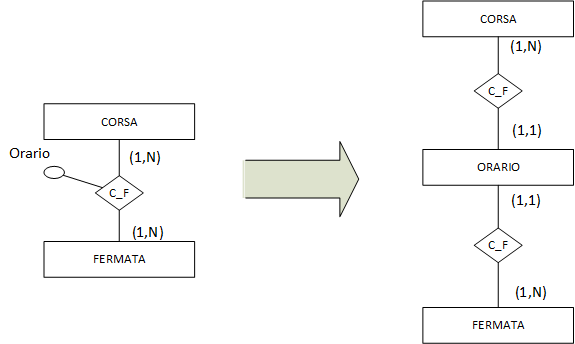
\includegraphics[scale = 0.3]{Modifica.png}
\caption{Modifica relazione}
\end{figure}

\chapter{Progetto Logico}
Il file ScriptProgBasi.sql rappresenta il progetto logico
\chapter{Popolamento}
Il file ScriptInserimento.sql rappresenta il popolamento della base di dati
\chapter{Progettazione Logica}
Il file page_schema.txt rappresenta i page schema del sito web

\end{document}